\documentclass[a4paper,man,natbib]{apa6}
\usepackage{microtype}
\usepackage{mathtools}
\usepackage{hyperref}
\usepackage{tabularx}
\newcolumntype{Y}{>{\raggedright\arraybackslash}X}

\usepackage[normalem]{ulem}
\hypersetup{hidelinks=true}
%\usepackage{lingex} % some linguistic-style example numbering


\newcommand*{\smex}[1]{\textit{#1}} % 'small example'
\newcommand*{\spex}[1]{``{#1}''} % 'spoken example'
\newcommand*{\term}[1]{\emph{#1}} % introducing a new term
\newcommand*{\citegen}[1]{\citeauthor{#1}'s~(\citeyear{#1})}
\newcommand*{\SE}{\mathit{SE}} % fix funny "SE" spacing
\newcommand{\resultsLog}[3]{$\beta = #1$, $\textnormal{SE} = #2$, $p #3$}
\newcommand{\resultsLM}[3]{$\beta = #1$, $\textnormal{SE} = #2$, $t #3$}


\title{Gestural cues to deception.}
\author{order(Martin Corley, Josiah P.\@ J.\@ King, Jia E.\@ Loy)}
\affiliation{Psychology, PPLS, University of Edinburgh}
\ifapamodeman{\note{\begin{flushleft}%
Josiah King\\
Philosophy, Psychology and Language Sciences\\
University of Edinburgh\\
7~George Square\\
Edinburgh EH8~9JZ, UK\\[1ex]
\url{J.P.J.King@sms.ed.ac.uk}
\end{flushleft}}}


%\shorttitle{What does a liar look like?}
\abstract{

Previous research shows links between body language and perceptions of deception. 
Traditionally, this is considered to stem from a form of speaker-modelling: lying takes cognitive effort, and effort is associated with certain visible gesticulations (e.g. scratching head, shifting position).
Recently, work has highlighted how listeners' associations between the manner of spoken delivery (speech disfluency) and dishonesty happen at the earliest stages of reference comprehension.
The studies presented here ask whether listeners also rapidly integrate the visual channel in making these pragmatic judgments.
Eye- and mouse-tracking experiments investigate the time-course of any associations listeners' might have between gestures and lying.

Participants saw and heard a potentially dishonest speaker describe treasure being hidden behind a named object, while also viewing both the named object and a distractor object. 
Their task was to click on the object behind which they suspected the treasure to actually be hidden.

Experiment 1 is an exploratory attempt to assess which, if any, types of gesticulations listeners might associate with deception, and investigates the potential obstacles to incorporating a video element into a visual world paradigm.

Experiment 2 establishes that listeners do associate gestures with deception, and that this happens at an early stage in reference comprehension.
Additionally, it examines whether listeners' judgments correlate with how nervous they think the speaker was in each video.
}

\noindent
%JK INTRO. 

\section{intro}

That people deceive one another is an inescapable aspect of everyday communication.
After recording participants' social interactions over a one week period, \citet{DePaulo1996} suggested that people lie on average twice a day.
The idea that there are systematic differences in people's behaviour depending on whether they are telling a truth or a lie has long captivated human interest in a variety of areas, from interrogations of criminal suspects to competition in the business world.\footnote{Where, in some cases, ``how to lie'' is equally as important. See https://www.marketplace.org/2008/02/18/business/lying-essential-doing-business}
Research suggests, however, that the behaviours which we associate with lying are often at odds with those behaviours which actually signal dishonesty.
A better understanding of this inconsistency, and of how listeners associate certain behaviour as signalling deceit, can shed light on our capacity to integrate non-verbal information during the on-line processing of speech.
The present experiments investigate the underlying biases which we might have about a speakers honesty and their non-verbal behaviour, and studies the time-course of such pragmatic judgments.

Much research has investigated the behaviours which listeners associate with a speaker's metacognitive states.
In speech, disfluency has been found to influence perceptions of both a speaker's certainty \citep{Swerts2005} and their honesty in an utterance \citep{Zuckerman1981, Loy2017}.
Interestingly, listeners appear to hold associations of disfluency with lying despite its accuracy deception-detection strategy being uncertain, with some evidence suggesting that lies are actually more fluent than truths \citep{Arciuli2009}.
In Loy20--?, listeners' disfluency-deception biases even persisted in the face of explicit feedback to the contrary.

In most natural communication, there are multiple channels of information on which to base a pragmatic judgment such as that of (dis)honesty: 
Lies may be discernable from truths in body-language and gestures as well as in speech.

The influence that being deceitful has on a speaker's movements may pattern with the influence it has on their spoken delivery: 
A reduction in illustrative gesturing has been associated with deceit \citep{DePaulo2003, Cohen2010}, as has both shorter talking time and a reduction in detail \citep{DePaulo2003}, suggesting that speakers are less informative --- in both speech and gesture --- when lying. 
%Cohen2010 found a few people gestured in ways which contradicted their lies - e.g. iconic gestures reveal our inner thoughts.
As speech contains disfluencies, the visual modality also contains a collateral channel, in the form of potentially unconscious movements and postures.
Research has found conflicting results in the relationships between such visual cues and deception, just as it has for speech disfluency (\citealt{Zuckerman1981, DePaulo2003}).
In some studies, evidence has suggested that deception is associated with a decrease in hand, arm, and leg movements \citep{DePaulo1992, Ekman1989, Vrij1995}, perhaps as a result of liars making efforts to control their behaviour.
In contrast, two meta-analyses (\citealt{Zuckerman1981, DePaulo2003}) found more movement (specifically shrugs and fidgeting) be indicative of deceit.
%also, perceived tension = indicative of deceit

However, just as there is a suggested disparity between listeners beliefs of what a liar sounds like and how a liar actually speaks, the same might be said of what a liar looks like.
Speakers' post-hoc perceptions of their own gesticulations when producing a lie have been found to be at odds with how they actually behaved:
\citet{Vrij1996} found that after partaking in two interviews --- one in which they were truthful, the other dishonest --- participants believed that their movements increased when lying, even though a decrease actually occurred.
Furthermore, whether or not participants were informed before-hand that deception is usually associated with a decrease in movements had no affect on subsequent beliefs about their own behaviour.

This disparity between actual and perceived cues to deception patterns with the consistent finding that we are bad at detecting lies from truths.
In reviewing 39 studies in detection of deception, \citet{Vrij2000} found an average accuracy rate of 56.6\% --- only just above chance. 
One suggested reason for this was that listeners often look for the wrong cues in attempting to detect deceit (as evidenced in \citealt{DePaulo1982}), perhaps resulting from being unaware of their own behaviour during lying (as in \citealt{Vrij1996}), combined with an inaccurate model of what deceitful behaviour looks and sounds like.

In order to better understand how listeners make these judgments, recent research by \citet{Loy2017} investigated the time-course of the disfluency-deception bias.
Using a visual world paradigm in which participants were presented with two objects, along with utterances describing the location of some treasure which was hidden behind one of the objects. 
These utterances were presented as having been elicited in a previous experiment, and could be either truthful or dishonest.
Crucially, \citet{Loy2017} manipulated the manner of spoken delivery, with half of the experimental items containing a speech disfluency.
Participants were tasked with choosing where they \textit{believed} the treasure to really be hidden --- the object named in the utterance (indicated a judgment of honesty), or the distractor (indicating dishonesty).
Participants judged disfluent descriptions of the treasure's location as more dishonest that fluent ones (as indicated by their choice of object).
Importantly, this corresponded to an early bias in both eye and mouse movements, suggesting that listeners integrate pragmatic information (such as the manner of spoken delivery) alongside the semantic content.
\citeauthor{Loy2017}'s findings contrast with more traditional views of language processing which prioritize interpretation of the literal content before accessing contextual information which might alter a message's global meaning.

Little is known, however, about whether this might extend to the visual channel.
Research into how speech and gesture interact in language comprehension has focused largely on how specifically illustrative gesture might influence the literal content of the message.
Gestures which mismatch accompanying speech have been found to interfere with comprehension in an on-line fashion, suggesting that speech and gesture are integrated in the real-time to form a unified system in comprehension (see \citealt{Kelly2010, Habets2013}).
The interplay between gesture and pragmatics, however, remains largely under-studied.
In the field of deception research, measuring listeners associations between movements and lying has been limited to post-hoc judgments, or assessing their explicit beliefs about the assocations (see \citealt{Vrij1996a, Zuckerman1981a}). 
The same is true of the few studies there have been outside of the deception literature, focusing on intentional gestures and their effect on the comprehension of, for example, indirect requests (see \citealt{Kelly1999}). 

The present studies develop the `treasure-game’ paradigm from \citet{Loy2017} to include a visual display of the speaker, manipulating the presence of gestures.
Experiment 1 attempts to assess which, if any, types of gesticulations listeners might associate with deception, and investigates the potential obstacles to incorporating a video element into a visual world paradigm.
In Experiment 2 we focus on if, how, and when, adaptor gestures (fidgeting movements) influence listeners' judgements of deception.
Additionally, we ask whether listeners' judgments are predicted by their perceptions of how nervous they think the speaker to be in each video.


%	GCD v1
\section{Experiment 1}
Eye- and mouse-tracking methods are used to investigate the time course of listeners' judgments about the honesty of an utterance, and how these judgments are influenced by the occurrence of various types of gestures. 
Specifically, we look at 3 types of gesturing, all of which have different (dis)advantages to consider when trying to integrate video in to a visual-world paradigm.
Visual-world studies typically present participants with a disembodied voice which produces expressions referring to a number of objects in a display which is visible to the participant.
Tracking participants eye-movements during this procedure allows researchers to study the time course of referential comprehension, and thus see how listeners' processing is influenced by a speaker's use of language.
However, the link between eye-movements and language processing is indirect: information in the presented speech affects participants' allocation of attention, which in turn regulates gaze position. 
The inclusion of a video component will likely draw more attention than the other, static, objects, potentially delaying or diminishing the detection of any on-line effects of gesture.

\subsection{Materials}
Visual stimuli consisted of the same 120 line drawings from \citet{Snodgrass1980} which were used in \citet{Loy2017}, presented in pairs across sixty trials. 
In each trial, the speaker named one object (referent) as that which concealed the treasure; the other object is hereafter named the distractor.
Each referent was associated with a recording specifying the image as the object that the treasure was hidden behind (``The treasure is behind the <referent>'').
Along with these images, each trial contained a video of a person who was purported to be the speaker of the utterances. 
So that videos could be counterbalanced across referents, and thus across utterances, the face of the person in the video was blurred. 
This meant that, when presented with a given utterance, it was believable that both audio and visual stimuli had been produced concurrently. 

Sixty videos (30 Gesture, 30 No-gesture) were created. 
The thirty no-gesture videos were comprised of ten recordings (each presented thrice) of a speaker sitting motionless with her hands either side of a tablet on a table, upon which the location of treasure was purported to be displayed.
Ten videos presented the speaker making one of five trunk movements, ten presented various adaptor gestures (e.g. finger tapping, head tilts), and ten presented the speaker sitting motionless but in a different position to that of the no-gesture videos (e.g. hand on chin, arms crossed, etc).

A selection of trunk gestures, adaptors (e.g. finger tapping, head tilts), and different postures, were used as gestural cues to deception.
Stimuli for this experiment had to strike a balance between being salient enough to register as a potential cue, but not being so distracting as to delay participants' fixating upon the images under discussion, thus losing any detection of possible on-line effects. 
The chosen selection balanced these two requirements in different ways.
Adaptor gestures, allowed for the most variation, but were required to overlap with speech in order to make the audio and video look believable.
This increased the potential for interference of the video at the point of the onset of the referent.
Trunk gestures were not susceptible to this, as they believable when the gesture was presented in its entirety prior to speech onset. 
Posture changes were presented in videos of the speaker sitting motionless but in a different position to that used in the no-gesture condition.
This meant that these videos were no more salient across the presentation of the utterance than the no-gesture videos.
However, because posture changes presented the speaker having implicitly shifted position at some earlier point, this ran the risk of weakening the association between the change of posture with the current utterance.

For each video of a trunk gesture, the frame at which the gesture ended was identified, and was the point at which the utterance began.
However, this meant that video-onset to speech-onset varied (Mean = 1430ms, sd=440ms), the duration of which could be interpretable as speech initiation time, which in turn could be associated with preparing a dishonest utterance.
To control for any effect of gesture being explained as simply a sensitivity to the duration of pre-utterance video, these durations were matched in the no-gesture videos.
For each of the adaptor gesture videos, the amount of overlap between speech and gesture was adjusted to make it as believable as possible that the two modalities were simultaneously produced (Mean = 1370ms, sd=410ms).
These durations were matched by the static posture shift videos.

Twenty referents were counterbalanced across two lists, each containing 10 trunk gesture videos, and 10 no-gesture videos. 
The remaining referents (40) were randomly paired with the remaining videos (10 adaptors, 10 static shifts, 20 no gesture) for each participant.
This was done only to match the structure of the previous treasure-game paradigm \citep{Loy2017}, with trunk gestures initially considered to be our best bet of eliciting gesture-dishonesty associations without interfering with the time-course of the judgment. 

\subsection{Procedure}
Stimuli were displayed on a 21~in.\@ CRT monitor, placed 850~mm from an Eyelink~1000 Tower-mounted eye-tracker which tracked eye movements at 500~Hz (right eye only). 
Audio was presented in stereo from speakers on either side of the monitor. 
Mouse coordinates were sampled at the frame rate of the videos (25~fps). 
The experiment was presented using OpenSesame version~3.1 \citep{Mathot2012}.

Participants were told that they were going to watch videos which were recorded from a previous experiment, in which one participant had to deceive another as to the location of some hidden treasure. 
Figure \ref{fig:v1trial} presents a sample trial from the experiment. 
\begin{figure}[Ht]
  \centering
	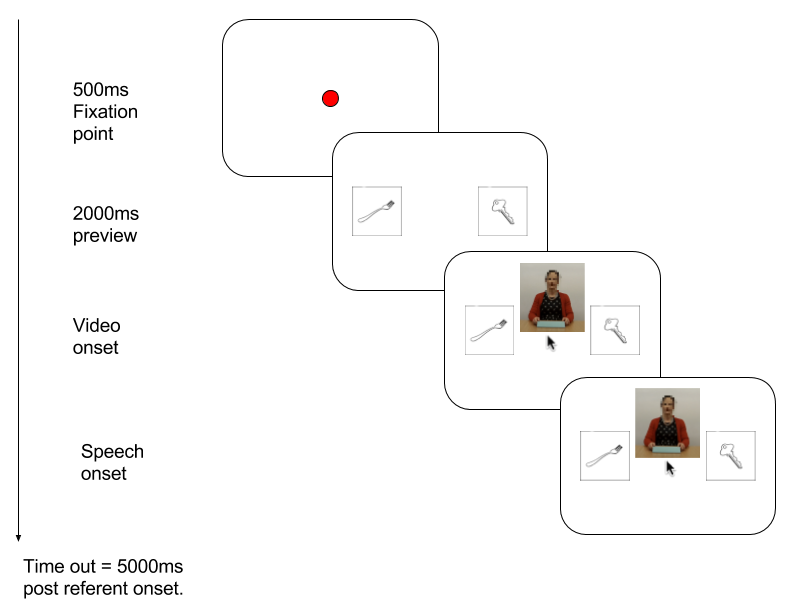
\includegraphics[width=\linewidth]{./img/gcdv1.png}
  \caption{Procedure of a given trial.}
  \label{fig:v1trial}
\end{figure}
Between trials, participants underwent a manual drift correct, after which the fixation dot turned red for 500ms. 
The two objects (referent and distractor) were displayed on the screen for 2000ms.
After this, the video appeared and the cursor was centred and made visible.
After a given time (M=1410ms, sd=410ms), the utterance began. 

\subsection{Bonus Rounds}
To maintain motivation throughout the study, participants were told that there were a number of ``hidden bonus rounds'' which offered more treasure. 
Following 25\% of the filler trials, a ``bonus round'' message appeared before progressing to the next trial.
This informed participants that they had successfully located bonus treasure (regardless of the object chosen).
Half of these appeared on randomly chosen trials in the gesture condition, and the other half in the no-gesture condition.

Participants were also told that the top scorers would be able to enter their names on a high-score table, which was shown at the beginning of the experiment. 

Participants completed five practice trials (one of which was presented as a bonus round) prior to the main experiment. 
Two of these were static, two displayed the speaker in different postures, and one displayed the speaker making a trunk gesture.

Eye movements, mouse coordinates and object clicked (referent or distractor) were recorded for each trial.

\subsection{Post-test Questionnaire}
Participants were asked to complete a short post-test questionnaire. 
The questionnaires contained three questions, the most important of which asked if participants noticed anything odd about the visual or audio stimuli.
Any participant who indicated that they noticed anything unusual was then verbally questioned, to decide whether they believed that the speech and gesture had been produced naturally and simultaneously.
All participants were subsequently debriefed (told that the audio and video were created separately and stitched together), and asked again verbally if they noticed anything unusual in that respect. 

\section{Results}
Twenty-four native English speaking participants took part in the experiment for a desired sample size of twenty. 
Participants were recruited from the University of Edinburgh community, and participated in return for a payment of \pounds{}4.
Four participants who indicated suspicion of the proposed origins of the audiovisual stimuli, and their data was removed from all analysis.

\subsection{Analysis}
Analysis was carried out in R version~3.4.3 \citep{Rbase2017}, using the lme4 package \citep{Bates2015}. 
Trials in which participants did not click on either the referent or distractor (0.003\% of trials) were excluded from all analyses. 

Analyses for both eye and mouse movements were conducted over a time window from 0 to 1200~ms after onset of the referent name.
Previous versions of this paradigm have tended to look at the period from 0 to 800~ms post referent-onset, this was lengthened for two reasons:
Firstly, analysis of previous versions considered a subset of referents, the longest of which was 776~ms, whereas the current experiment includes all referents, with the longest at 1062~ms.
Secondly, we expected the inclusion of the video component to distract ---- and so to delay --- listeners from fixating to either referent or distractor.

Eye fixation data was averaged into 20~ms bins (of 10 samples) prior to analysis.
For each bin, we calculated the proportions of time spent fixating referent or the distractor, resulting in a measure of the proportions of fixations on either object over time.

The position of the mouse was sampled every 40~ms.
Using the $X$ coordinates only, we calculated the number of screen pixels moved and the direction of movement (towards either referent or distractor).
We then calculated the cumulative distance travelled towards each object over time as a proportion of the cumulative distance travelled in either direction.
%JK Movements beyond the outer edge of either object were considered to be `overshooting' and were not included in calculations (???\% of samples).
Eye- and mouse- biases were calculated from the proportions of referent to distractor fixations, and were subsequently empirical logit transformed \citep{Barr2008}, 
In these measures, a value of zero indicates no bias towards either object, and positive and negative values indicate a bias towards the referent and distractor respectively.

Eye and mouse data was modelled over the window of 200 to 1200~ms post-referent onset using linear mixed effects models, with fixed effects of time, gesture type (No Gesture, Posture change, Trunk movement, Adaptor), and their interaction.
Random intercepts and slopes for time by-referent were included, along with random intercepts and slopes for time, gesture type and their interation by-participant.
Following \citet{Baayen2008}, we considered effects in these models to be significant where $|t|>2$.

The object clicked (referent or distractor) was modeled using mixed effects logistic regression, with fixed effects of gesture type and random intercepts and slopes for gesture type by-participant and random intercepts by-referent.
Reaction times (measured from referent onset) were modelled with the same fixed and random effect structure, also with mixed effects logistic regression.
Following \citet{Lo2015}, we compared models which specified an identity link function, assuming gaussian, gamma and inverse gaussian distributions. 

\subsection{Object clicks}
when presented with an utterance accompanied by no-gesturing, participants showed a bias toward a final interpretation of the utterance as truthful, with more clicks to the referent than the distractor \resultsLog{0.61}{0.15}{<0.001}.

all types of gestures saw a reduction in this bias, with adaptor gestures (\resultsLog{-1.01}{0.36}{<0.005}) showing a greater change than posture change and trunk movements (\resultsLog{-0.70}{0.30}{<0.05} and \resultsLog{-0.61}{0.26}{<0.05} respectively).

\subsection{Reaction times}
Model comparison of both AIC and BIC found that assuming an inverse gaussian distribution provided the best fit to the observed data.
Participants responded to videos displaying a trunk movement faster than they did to no-gesture videos (\resultsLog_ns{-87.17}{34.32}{<0.05}).
Responses to videos showing adaptor gestures showed a marginal effect in the same direction (\resultsLog_ns{-61.17}{33.65}{=0.07}).
%% it's interesting, because these are the two conditions in which there is a movement. there's a small amount of research >> Holler 2017: Processing language in face-to-face conversation: Questions with gestures get faster responses.
%but it seems less intuitive an effect in this context because the gesture is not contributing info in the same way. 
% I'd be interested to look at all the studies we've done with gestures in visual world, and see whether moving = faster across the board. I think it might. although.. hopefully not for the mismatched gestures??

\subsection{Eye movements}
Figure \ref{fig:eye} shows the time-course of fixations to referents and distractors over 2000~ms from referent onset, split by each type of video.
Analyses conducted over the period from referent onset to 1200~ms post onset showed that, when presented with no gesture, participants displayed an early fixation bias towards the referent, which increased over time (\resultsLM{}{}{}).


\subsection{Mouse movements}

\section{Discussion}



There were several things to note from version 1. 
Firstly, the gestures used in the filler trials (adaptor gestures, often involving hands) appeared to bias participants more strongly towards an eventual interpretation of dishonesty than the critical gestures (trunk movements). 
This could be simply that the filler gestures were more visually salient than trunk movements, resulting in participants attending towards the speaker’s hands more than to her trunk.
Alternatively, it could be that listeners do not associate trunk movements with deception, contra previous research (Vrij, 2000)

Several participants reported post-test that in making their judgments, they were assessing “how relaxed” the speaker looked during the utterance. 
This led us to rethink our justification for the type of gesture which we would expect to elicit judgments of dishonesty. 
In the current version (version 2) we make the following line of reasoning: If listeners are reasoning (perhaps via introspection) about what lying involves (e.g. effort, nervousness, etc.), then gestures which are likely to function as cues to deception should reflect this  reasoning.

An additional comment from several participants was that they sometimes considered the no-gesture videos to show the speaker looking more unrelaxed.
This is something we had not considered, and we attempted to make the no-gesture videos for version 2 look more relaxed (more slumped/slouched posture).




% GCD v2
\section{Experiment 2}
%JK summarise differences/motivations
same as experiment 1 only reduced set (no filler trials), constant speech onset latency, just adaptor gesture, 


Based on Gregerson (2005), we use adaptor gestures as our critical gestures. 
Adaptors are typically associated with nervousness, and include various hand and arm gestures such as finger taps, fidgeting, rubbing shoulders etc. 

Additionally, all videos are rated by 10 naive volunteers for “how nervous the speaker looks” prior to running the study.
Post-test, participants will be asked to rate a selection of videos (both gesture and no-gesture) for nervousness.
Key differences between version 1 and version 2.
Version 2 contains no filler trials.
Version 1 contained 40 filler trials with various gestures, which in hindsight served no purpose. In fact, they contained the very types of gesture which are likely to be a) more salient and b) more strongly associated with lying (given an introspection speaker modelling account).
Version 2 = 20 trials long. Practice trials changed from 5 to 4.

Critical gestures are adaptors (as opposed to trunk movements in version 1)
A result of this is that in version 2 there is gesture/speech overlap, whereas in version 1 there was no overlap. This might cause problems as participants may fixate more to the gesturing than to the objects at the relevant time (referent onset).
No-gesture videos show the speaker in a more relaxed posture.
All videos rated (n=10) for nervousness prior to study.
Video onset to speech onset is a constant (rather than a variable matched across conditions)
Participants rate videos for nervousness post-test.

%jk done below. not done above.
\subsection{Materials}
A subset of 40 images from those in Experiment 1 were used across twenty trials.
As in Experiment 1, these images were presented in referent-distractor pairs, combined with 20 utterances naming the referent as the location of the treasure.
The referents and distractors used were those which, in \citet{Loy2017}, had been matched for both ease of naming and familiarity.

In Experiment 2, participants saw these pairs of images alongisde one of 20 videos: 10 Gesture, and 10 No-gesture.
The videos in the gesture condition showed the speaker making some form of adaptor gesture (tapping fingers, twirling hair, rubbing shoulder, etc).
Table \ref{table:gestures} shows a breakdown of the different gestures used.

\begin{table}
\caption{Gestures used}
\label{table:gestures}
\begin{tabularx}{\linewidth}{YY}
\hline
& Number \\
\hline
\textbf{Block 1} & \\
finger scratch & 220\\
hair twirl & 220 \\
\hline
\end{tabularx}
\end{table}


The 10 no-gesture videos showed the speaker sitting motionless, with special care taken to present a relaxed posture.
Prior to running the experiment, all videos were rated on how nervous the speaker looked.
10 native english speakers were told that they were going to watch videos (without audio) of someone being questioned in a stressful situation, and were asked to rate how nervous the speaker looked in each video (1: very relaxed, 7: very nervous). 
Gesture videos were rated as more nervous (Mean = 4.1, SD = 1.5) than the no-gesture videos (M = 1.9, SD = 1.1).

The 20 referents were counterbalanced across two lists, each containing 10 gesture videos, and 10 no-gesture videos, such that each referent that occurred with a gesture video in the first list occurred with a no-gesture video in the second.
The pairings of referents with specific videos in each condition was randomised on each run of the experiment.

In Experiment 2, speech initiation time (the duration from video onset to speech onset) was controlled in the experimental design. 
In all trials, the speech began 1170~ms after the beginning of the video.
This was the only procedural difference in trials between experiments 1 and 2 (see \ref{fig:v2trial}).

Figure \ref{fig:v2trial} presents a sample trial from Experiment 2. 
\begin{figure}[Ht]
  \centering
	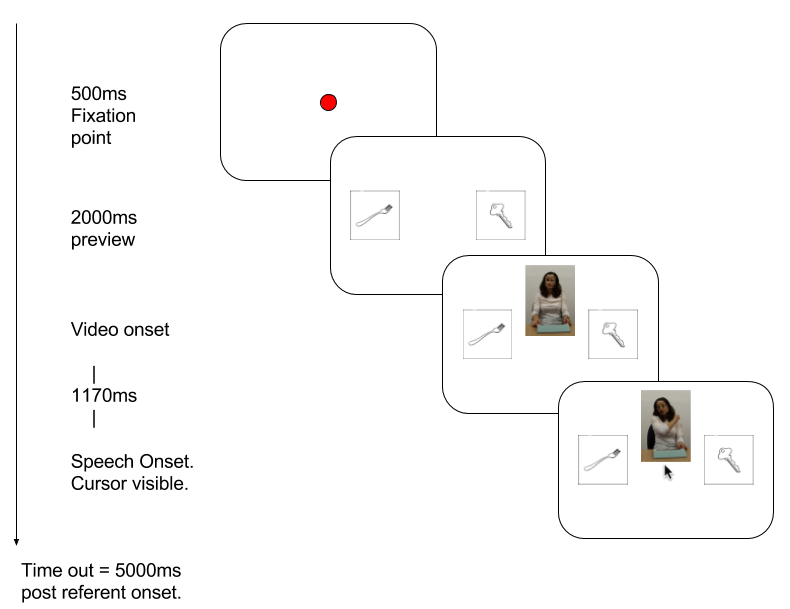
\includegraphics[width=\linewidth]{./img/gcdv2.png}
  \caption{Procedure of a given trial.}
  \label{fig:v2trial}
\end{figure}

After the main task, participants were asked to watch the videos again, without audio, rating how nervous they thought the speaker looked (using the same 1-7 scale as described above).

Participants then completed the same post-test questionnaire as in Experiment 1, and data was excluded from analysis based on the same criteria.

\subsection{Analysis}
%JK same as for v1
%JK what about the ratings?

\subsection{results}
\subsubsection{Object click}
\subsubsection{Eye movements}
\subsubsection{Mouse movements}

\subsection{gen. discussion}


\bibliography{/home/josiah/Documents/bibtex/GCD}


\end{document}
